%!TEX root=../../../main.tex

Kravet til pH-proben er at den skal virke omgående når der hældes gødning i vandet. Dette vil sige at den skal omgående kunne fortælle systemet når der er den korrekte pH-værdi, når der doseres gødning. Efter nogle søgninger på Google blev der fundet frem til at en glasprobe var det meste effektive, men samtidig og så det billigste. 

\begin{figure}[H]
	\centering 
	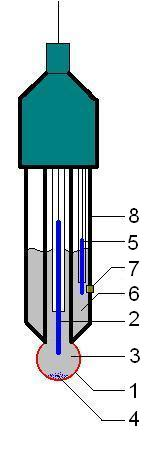
\includegraphics[scale=0.7]{HardwareArkitektur/Sensore/pH_probe_billeder/Glass_electrode_wiki.jpg}
	\caption{Tegning af en glasprobe. kilde: Wikipedia}
	\label{photo:pH-probe}
\end{figure}     

pH værdi er en måde at angive hvor mange hydrogen-ioner der er i væsken. Definitionen af en syre er at den modtager hydrogen-ionerne og definitionen af en base er at den afgiver hydrogen-ioner. Vand kan både optræde som en syre og en base, dette skyldes at vand vil modtage hydrogen-ionerne når der hældes en base i, men det vil afgive hydrogen-ioner når der hældes en syre i. På figur \ref{photo:pH-skala} ses at har vi $10^{-14}$ mol/l af H+ ioner har vi en pH-værdi på 14. 

 \begin{figure}[H]
	\centering 
	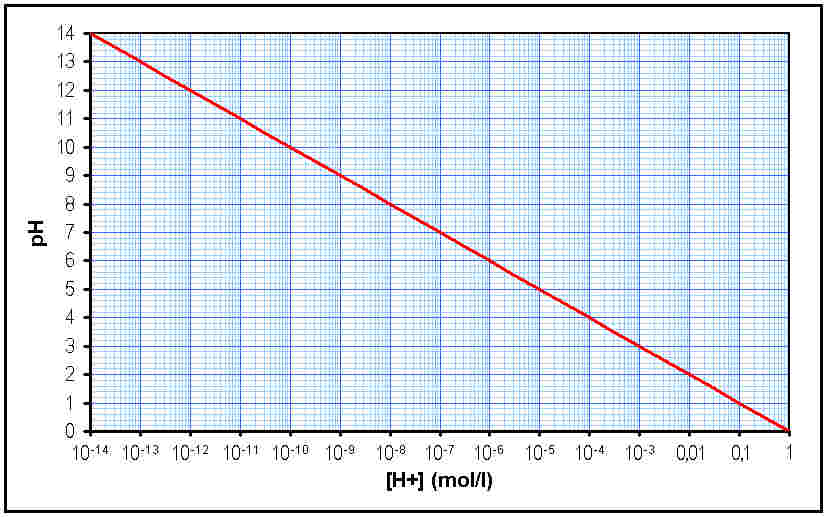
\includegraphics[scale=0.4]{HardwareArkitektur/Sensore/pH_probe_billeder/PH-skala.jpg}
	\caption{Graf over pH-værdi. kilde: Wikipedia}
	\label{photo:pH-skala}
\end{figure}   

Måden glasproben virker på at at den internt er fyldt op med saltsyre HCL. I figur \ref{photo:pH-probe} punkt 3 er koncentrationen $1*10^{-7}$ mol/l. I punkt 6 er koncentrationen $0.1$ mol/l. På denne måde bliver der genereret en spænding når der er et overskud eller underskud af H+ ioner på ydersiden af punkt 1. H+ ionerne vil tiltrække CL- ionerne som ses i punkt 4. Punkt 2 og 5 er elektroderne som vi måler spændingen over. I figur  \ref{photo:probeslope} ses outputtet fra proben i forhold til pH-værdien i den væske den er i. 

 \begin{figure}[H]
	\centering 
	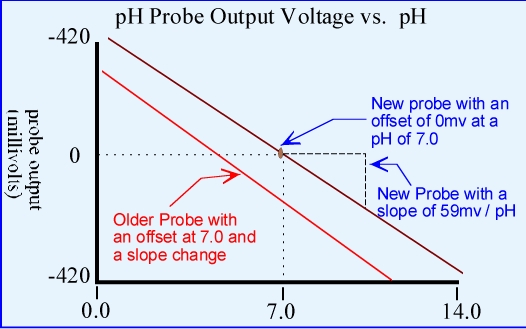
\includegraphics[scale=0.4]{HardwareArkitektur/Sensore/pH_probe_billeder/probeslope.jpg}
	\caption{Outputtet fra pH-proben}
	\label{photo:probeslope}
\end{figure} 

For at få en præcis måling af væsken kræver det at der laves en kaliberering af pH-proben en gang hver måned, da proben vil drifte med tiden. Det ses også på figur \ref{photo:probeslope} at en ny probe vil give en højrer spænding en en ældre. Dette betyder at den skal kalibreres en gang i mellem. Til kalibrering af proben skal der bruges noget buffervæske. En buffervæske er en væske med en præcis pH-værdi således at proben kan indstilles efter det. Måden vi vil gøre det på er ved at have en buffer med pH-værdi 7. Når systemet startes op skal proben kalibreres og der vil være en rød LED på karet der lyser. For at kalibrere proben sættes proben ned i buffervæsken og efter ca 30 sekunder trykkes der på en knap som sidder på karet og karet indlæser herved værdien til kalibrering. På figur \ref{photo:buffer_vaeske} ses at buffervæsken varierer sin pH-værdi ved temperaturforskelle. Dette vil også være gældende for andre væsker, dette er ikke noget vi tager højde for i vores målinger, men det burde blive implementeret i et salgsklart system. 

 \begin{figure}[H]
	\centering 
	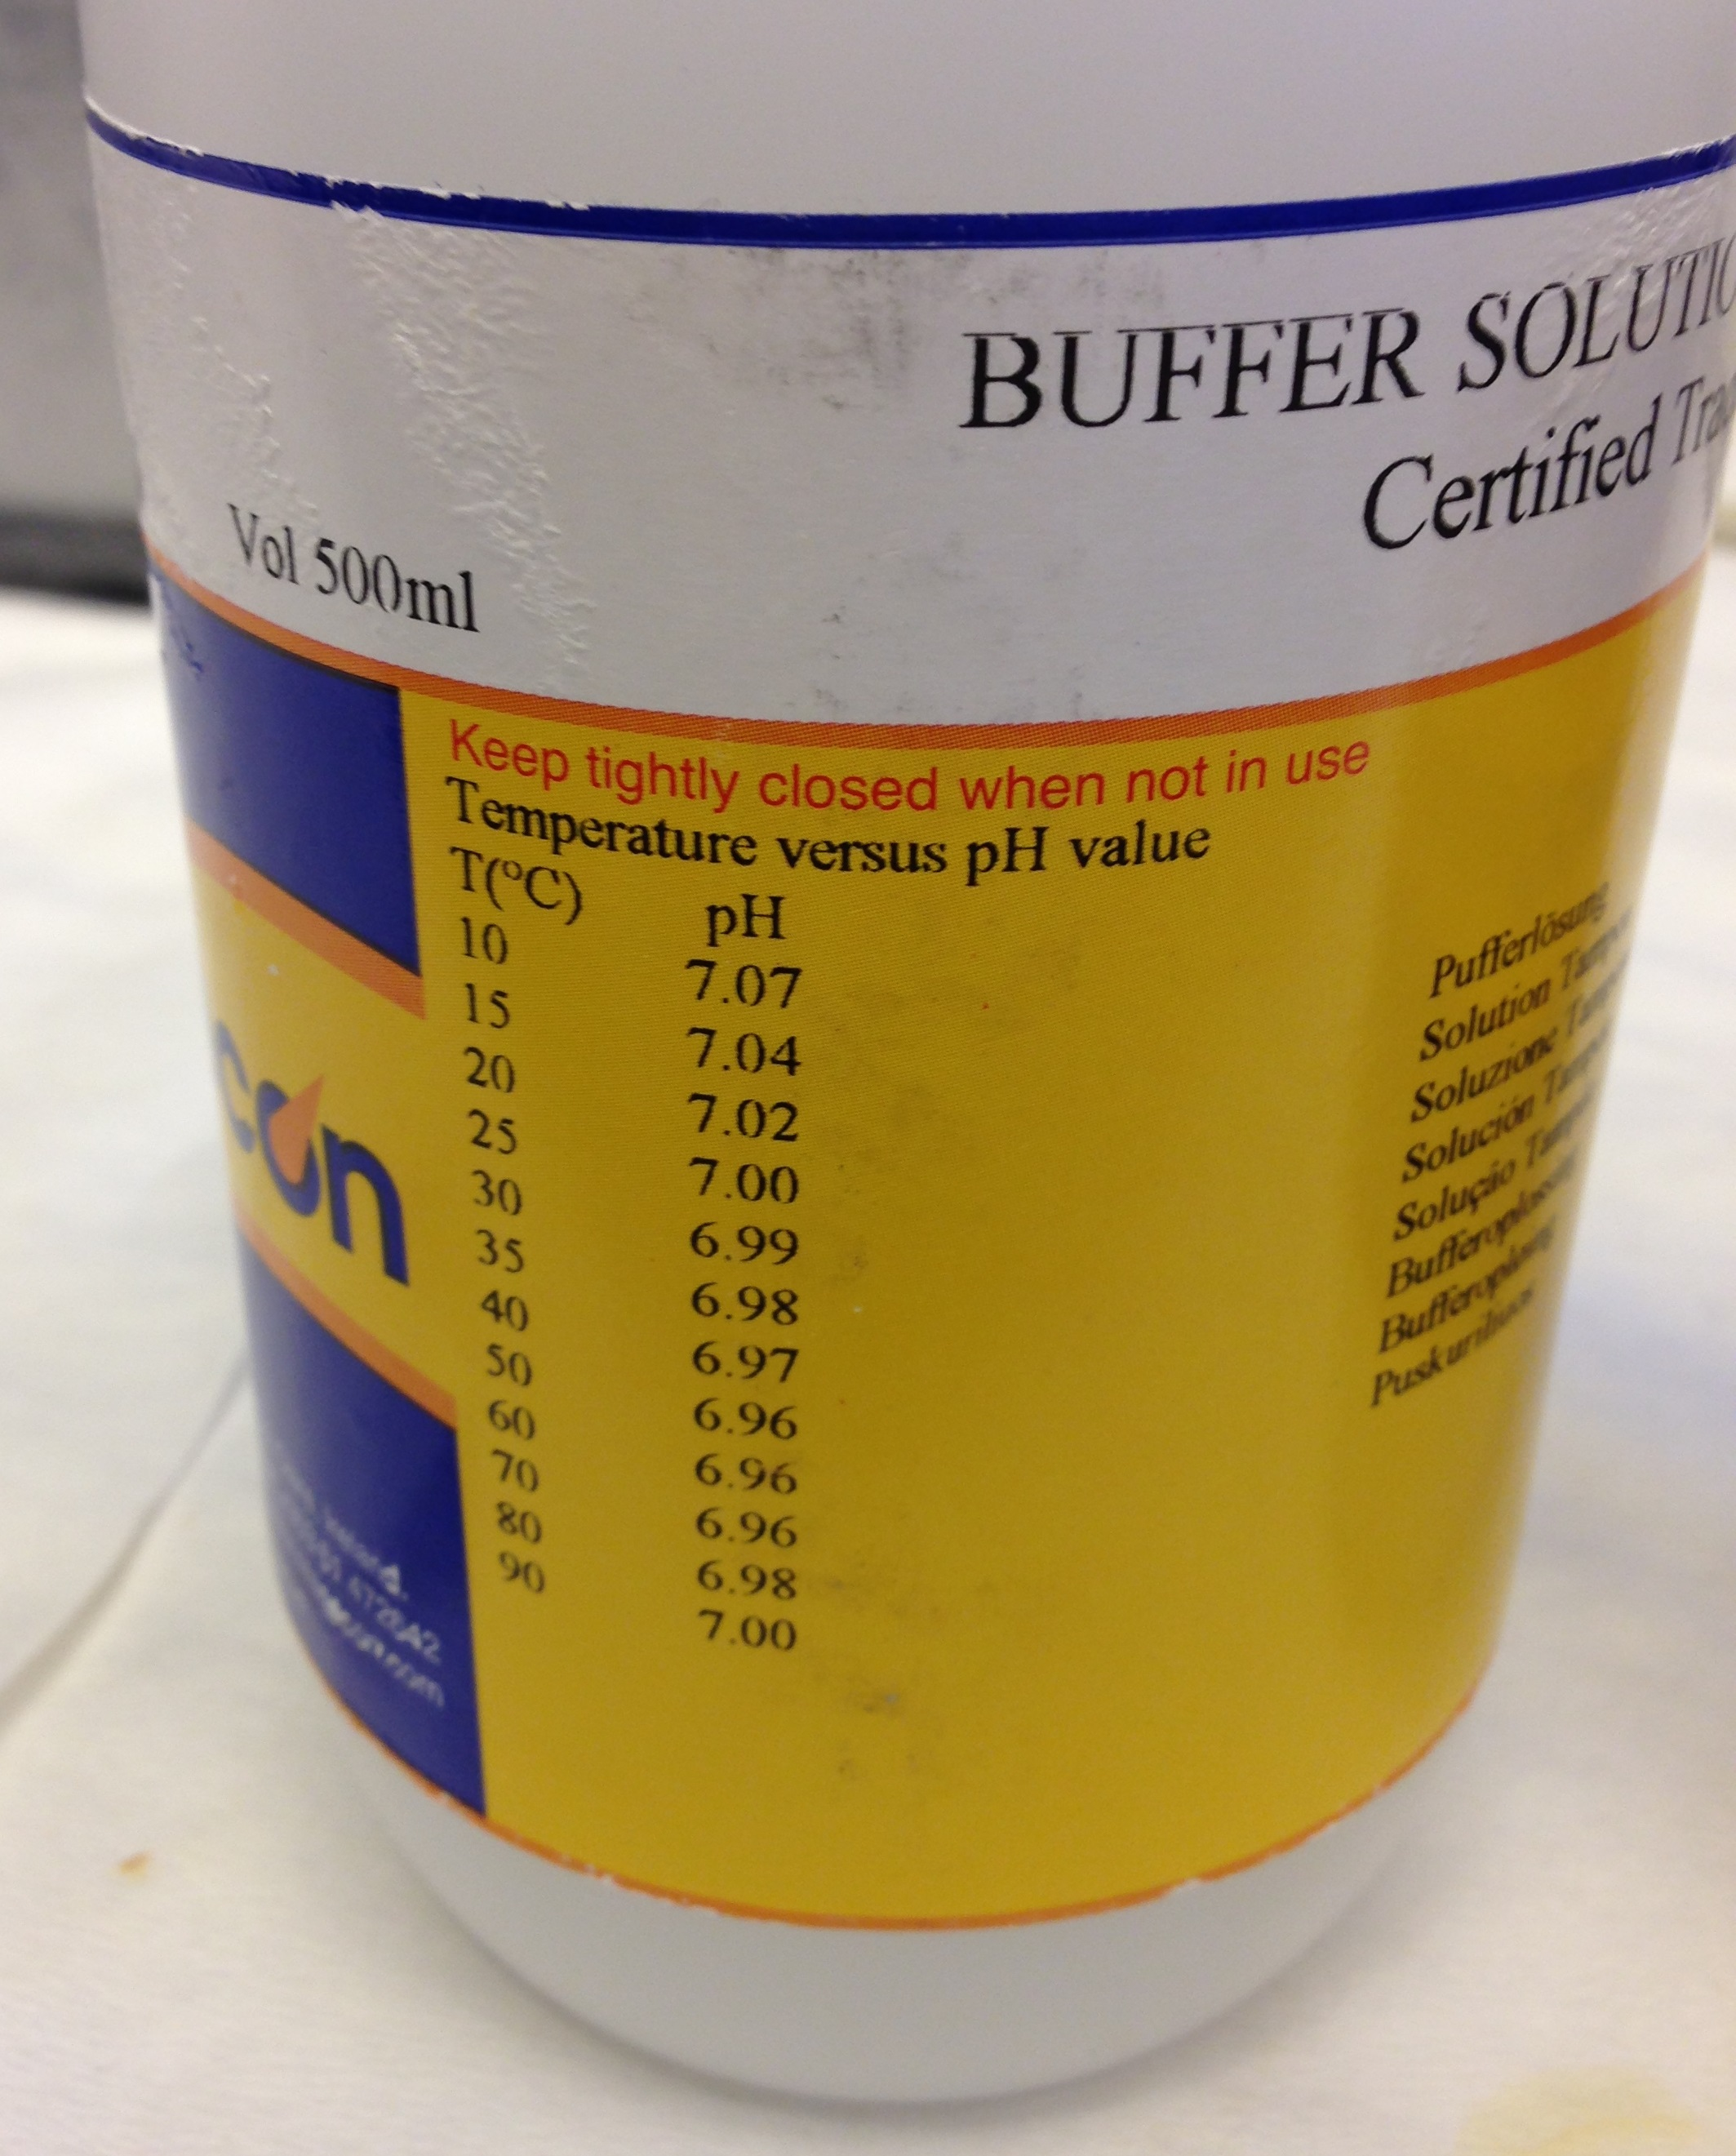
\includegraphics[scale=0.1]{HardwareArkitektur/Sensore/pH_probe_billeder/buffervaeske.jpg}
	\caption{Temperaturens indflydelse på pH-værdien i buffervæsken}
	\label{photo:buffer_vaeske}
\end{figure} 
Nedenfor ses koden til pH-proben. Koden er klar til at blive implementeret i kar-softwaren. Men for overskuelighedens skyld vælges det at vise den individuelle kode her. Der er oprettet en funktion getPhVal() som returnerer pH-værdien.

\lstinputlisting[language=c]{HardwareArkitektur/Sensore/kode/pH_kode.txt} 

\subsection{Støj}

For at få en præcis måling vælger vi at analysere proben for dens støj. Dette gøres ved at lave et nyt PSoC projekt. I Mixed Signal Electronic's har vi arbejdet med dette og vi kopierer derfor et kredsløb derfra. Det skal dog siges at projektet er til PSoC5 og her i Projektet bruger vi en PSoC4. PSoC5 har den fordel at den har en DeltaSigma ADC som er bedre til at sample lavfrekvente signaler. I PSoC4 er den eneste mulighed en SAR converter. På figur \ref{photo:Topdesign_stoj} ses topdesignet i PSoC creator. 
 \begin{figure}[H]
	\centering 
	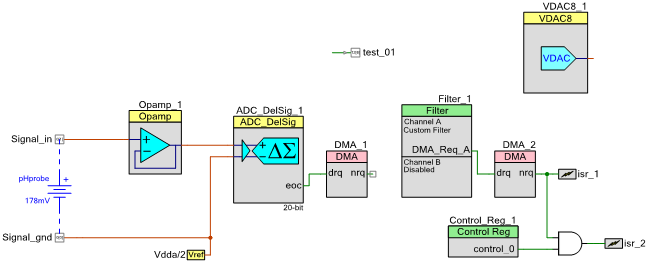
\includegraphics[scale=0.8]{HardwareArkitektur/Sensore/pH_probe_billeder/Topdesign_stoj.png}
	\caption{Topdesign i PSoC creator over kredsløbet til støjmåling}
	\label{photo:Topdesign_stoj}
\end{figure} 

For at kunne beregne støjen fra proben skal vi måle dens indre modstang og derefter bruge Johnson Nyquist formel for termisk støj. 
$$ V_n = \sqrt{4*K*T*R*\Delta f} $$

For at måle den indre modstand i proben kobler vi den med en buffer i PSoC4. Vi prøvede at måle selve indgangsimpedansen i bufferen da den ikke var opgivet i databladet. Dette var desværre ikke muligt da støj på indgangen fik den til at klippe på udgangen. Vi antager derfor at indgangsimpedansen er uendelig og kan for at måle udgangsspændingen ubelastet, opstille kredsløbet i figur \ref{photo:Non_inv_buf}. 

 \begin{figure}[H]
	\centering 
	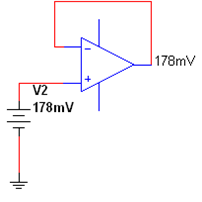
\includegraphics[scale=1]{HardwareArkitektur/Sensore/pH_probe_billeder/Non_inverting_buffer.png}
	\caption{Non-inverting buffer}
	\label{photo:Non_inv_buf}
\end{figure} 

Der måltes 178mV på udgangen af bufferen med proben sat ned i en buffervæske med en pH-værdi på 4. Derefter blev proben sat direkte i oscilloskopet som har en indgangsimpedans på 1M\ohm . Nedenstående kredsløb opstilles for denne måling figur \ref{photo:Kredslob_RI}. 


 \begin{figure}[H]
	\centering 
	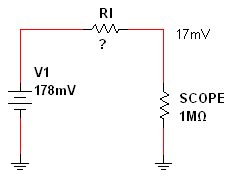
\includegraphics[scale=1]{HardwareArkitektur/Sensore/pH_probe_billeder/Kredslob_RI.png}
	\caption{Diagram over den indre modstand}
	\label{photo:Kredslob_RI}
\end{figure} 

Vi udregner med ohms lov den indre modstand til at være 9.5M\ohm . Vi kan derfor udregne støjbidraget til at være
$$ V_n = \sqrt{4*1.3806488*10^{-23}*297*9.5*10^{6}*100} = 3.9uV $$
Selve bufferen har også et støjstrøms bidrag som vil resultere i en støjspænding over modstanden i proben. Vi har i MSE øvelse 5 arbejdet med disse støjstrømme og kan pga. viden derfra antage at bufferen bidrager med $5pA$ i støjstrøm. I PSoC bruger vi et digitalt filter på 100Hz. Vi ville gerne have kørt det ned til 1Hz, men det mindste vi kunne implementere var 100Hz.
$$ V_n = I_{rms}*R_i*\sqrt{\Delta f} = 5pA*9.5M\ohm *\sqrt{100} = 475uV $$
Støj fra bufferen:
$$ V_n = 1.3uV * \sqrt{100} = 13uV $$
Støj fra ADC'en:
$$ V_n = 10uV * \sqrt{100} = 100uV $$
For at addere støjbidragene adderer vi dem kvadratisk da vores værdier er RMS støj:
$$ V_{ntot} = \sqrt{3.9uV^2 + 475uV^2 + 13uV^2 + 100uV^2} = 485uV $$
Det ses at det største og mest betydende støjbidrag er støjstrømmen fra bufferen. 

\subsubsection{Måling af støj}

For at måle støjen åbner vi teraterm og udlæser værdien. I projektet er der lavet funktioner til at skrive støjværdierne ud. For at måle den samlede støj sættes proben ned i en buffervæske med pH-værdi = 4. På figur \ref{photo:stoj_teraterm} ses en måling af den samlede støj på ca 4.8mV.

 \begin{figure}[H]
	\centering 
	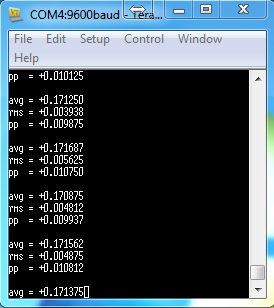
\includegraphics[scale=1]{HardwareArkitektur/Sensore/pH_probe_billeder/stoj_teraterm.png}
	\caption{Udlæsning på teraterm}
	\label{photo:stoj_teraterm}
\end{figure} 

 \begin{figure}[H]
	\centering 
	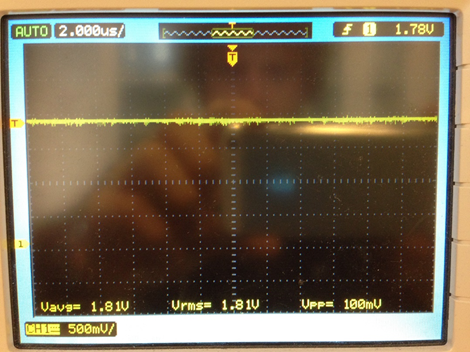
\includegraphics[scale=0.9]{HardwareArkitektur/Sensore/pH_probe_billeder/stoj_oscilloscope.png}
	\caption{Måling fra DAC'en på scopet}
	\label{photo:stoj_scope}
\end{figure} 

\subsubsection{Responstid}
For at måle responstiden, sættes proben i en buffer 7 og derefter direkte over i en buffer 4. Da H+ ionerne stadig vil sidde på proben når den trækkes op af buffer 7, sker der først en reaktion når den kommer ned i buffer 4.  Denne respons ses på figur \ref{photo:respons} . Her aflæses responstiden til 1.4 sekunder.

 \begin{figure}[H]
	\centering 
	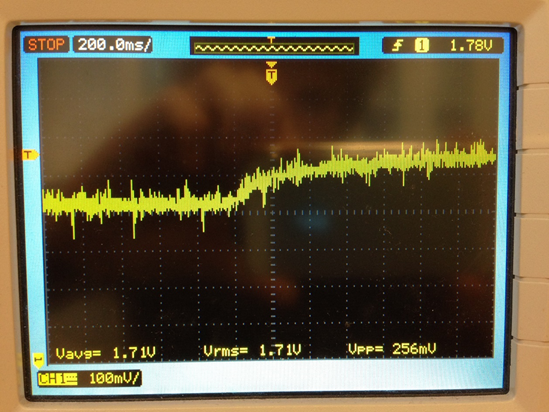
\includegraphics[scale=0.8]{HardwareArkitektur/Sensore/pH_probe_billeder/respons.png}
	\caption{Responstiden fra proben}
	\label{photo:respons}
\end{figure} 

\subsubsection{Probens præcision}
Selve proben vil have en afvigelse. Denne afvigelse tages der tildels højde for ved kalibreringen, men dette er kun den systematiske fejl der bliver reguleret ind. Der vil også være et antal tilfældige fejl, som vil være umulige at justere ind. For at få et overblik over fejlprocenten laver vi 10 målinger efter kalibrering af buffer 7. Her sætter vi proben ned i en kop vand, for derefter at sætte den ned i pH-bufferen igen. Vi venter i 2 minutter og aflæser derefter i debuggin mode hvad pH-værdien er. Målingerne skrives ind i et excel-regneark således vi kan udregne standardafvigelsen ved en konfidens på 95. Det skal dog siges at dette er en meget simplificeret metode, da der her ikke taget højde for temperatur forskelle. Der laves også kun 10 målinger ved en bestemt pH-værdi. Der burde laves målinger over hele aksen, for at dække usikkerheden helt ind.    

 \begin{figure}[H]
	\centering 
	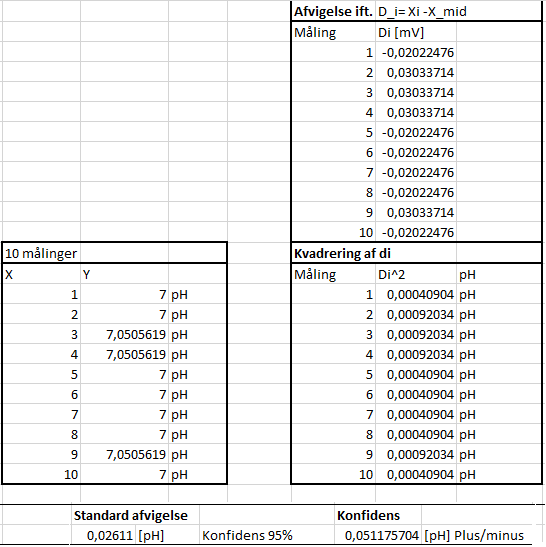
\includegraphics[scale=1]{HardwareArkitektur/Sensore/pH_probe_billeder/Probe_afvigelse.PNG}
	\caption{Probens præcision}
	\label{photo:probe_afvigelse}
\end{figure} 

Det ses at vi med 95\% sikkerhed kan sige at den målte værdi ligger inden for +-0,051175704 i pH-værdi, men som nævnt tidligere er dette ikke en endelig præcision.    

\subsubsection{Fremtidigt arbejde}
Vi så i denne del at vores beregnede støj var ca en faktor 10 større ved realiseringen end beregningerne. Dette kan skyldes at der er støj i tilledningerne da vi arbejder med ekstremt høje impedanser. Vi kan hermed konkludere at ved meget høje impedanser bliver ens udstyr meget støjfølsomt og det er derfor vigtigt at tage det med i beregningerne når der udlægges print, samt ved beslutning om hvilken terminering der skal benyttes. Fremtidigt arbejde kan være at lave kalibreringsfunktionen således den selv giver besked, når der er gået en måned, om at det er tid til kalibrering. 



